\documentclass[11pt, oneside]{article}   	% use "amsart" instead of "article" for AMSLaTeX format
\usepackage{geometry}                		% See geometry.pdf to learn the layout options. There are lots.
\geometry{letterpaper}                   		% ... or a4paper or a5paper or ... 
%\geometry{landscape}                		% Activate for for rotated page geometry
%\usepackage[parfill]{parskip}    		% Activate to begin paragraphs with an empty line rather than an indent
\usepackage{graphicx}				% Use pdf, png, jpg, or eps� with pdflatex; use eps in DVI mode
								% TeX will automatically convert eps --> pdf in pdflatex		
\usepackage{amssymb}
\usepackage{amsmath}

\title{Minmax problems in multi-variable calculus}
%\author{The Author}
%\section{}
% \subsection*{R code}
\date{}							% Activate to display a given date or no date

\graphicspath{{/Users/telliott_admin/Dropbox/Tex/png/}}

% \begin{center} 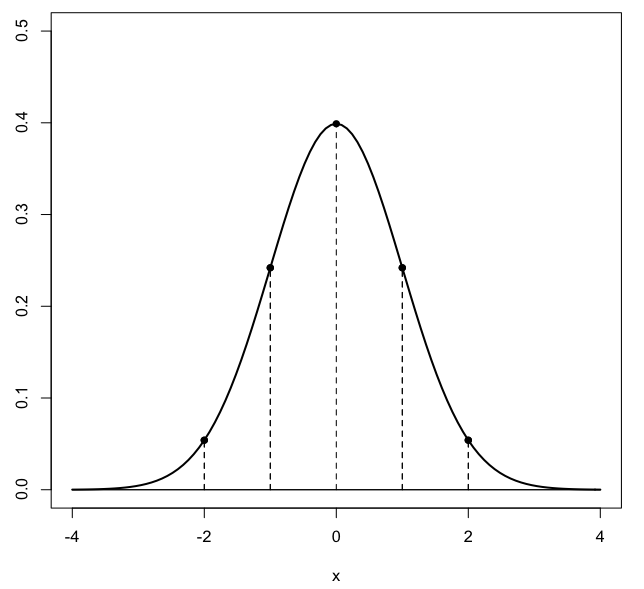
\includegraphics [scale=0.4] {gauss3.png} \end{center}
% \begin{bmatrix} a  &  b \\ c  &  d \end{bmatrix}
% \bigg |_

\begin{document}
\maketitle
\large
%\noindent
\subsection*{Two simple examples}

Suppose that we have three variables $x,y,z$ and we know that 
\[ x + y + z = 120 \]
We want to find solve this subject to the constraint that $xyz$ is a maximum.  Now, this problem really has only two variables, because once we have picked $x$ and $y$ we know $z$
\[ z = 120 - x - y \]
Our function $f(x,y)$ is then
\[ P = f(x,y) = xyz = xy(120-x-y) \]
We want to find the critical points of this function, and determine which is a maximum.  To do this, we take the partial derivatives
\[ f(x,y) = 120 xy - x^2y - xy^2 \]
\[ f_x = 120 y - 2xy - y^2 \]
By symmetry
\[ f_y = 120 x - 2xy - x^2 \]
We set $f_x=0$ and $f_y=0$
\[ 0 = 120 y - 2xy - y^2 \]
\[ 0 = 120 x - 2xy - x^2 \]
We notice that we can factor out a single $x$ or $y$
\[ y(120 - 2x - y) \]
\[ x(120 - 2y - x) \]
So obviously $x=0$ and $y=0$ are critical points, but also we are at a critical point if
\[ 120 - 2y - x = 0 \]
\[ 120 - 2x - y = 0 \]
We can solve this system
\[ 120 - 2y - x = 120 - 2x - y \]
\[ - 2y - x = - 2x - y \]
\[ - y = - x  \]
\[ x = y  \]
\[ 120 - 2x - x = 0 \]
\[ x = y = 40 \]
\[ z = 120 - x - y = 40 \]
This appears to be a maximum because
\[ x^3 > (x-1)(x+1)x = x^3 - x\]
for all $x > 0$
\vspace{5 mm}

\noindent
A problem that looks different at first but works in a similar way is the following.  Consider the plane that goes through the x-axis at (6,0,0), the y-axis at (0,4,0) and the z-axis at (0,0,3).  By substitution, we can see that the following equation is the equation of this plane.
\[ 2x + 3y + 4z = 12 \]
Construct a rectangular box with one corner at the origin and the other corner at $(x,y,z)$, subject to the constraint that $x,y,z$ is in this plane.  Pick $x,y,z$ to give the maximum volume.  We know that
\[ z = \frac{1}{4}(12 - 2x - 3y) \]
\[ V = f(x,y) = xyz = xy \  \frac{1}{4}(12 - 2x - 3y \]
\[ = 3xy- \frac{1}{2} x^2y - \frac{3}{4}xy^2 \]
This is quite similar to the first problem, except for the cofactors, which leads to a solution that is not symmetrical in $x,y,z$.  Take the partial derivatives, factor if possible, and set them equal to 0.
\[ f_x = 3y- xy - \frac{3}{4}y^2 \]
\[ = y(3 - x - \frac{3}{4}y) = 0 \]
\[ f_y = 3x - \frac{1}{2} x^2 - \frac{3}{2}xy  \]
\[ = x(3 - \frac{1}{2} x - \frac{3}{2}y )  = 0\]
As before, one set of critical points is where $x=0$ or $y=0$ but these are minima.  To solve, let's set the two derivatives (without the factors $x$ or $y$) equal to each other
\[ 3 - x - \frac{3}{4}y = 3 - \frac{1}{2} x - \frac{3}{2}y \]
\[ x + \frac{3}{4}y =  \frac{1}{2} x +\frac{3}{2}y \]
\[ \frac{1}{2}x =  \frac{3}{4}y \]
\[ x = \frac{3}{2} y \]
Back substituting
\[ 3 - \frac{1}{2} x - \frac{3}{2}y = 0 \]
\[ 3 - \frac{3}{4} y - \frac{3}{2}y = 0 \]
\[ 1 - \frac{3}{4} y = 0 \]
\[ y = \frac{4}{3}  \]
\[ x = \frac{3}{2} y = 2  \]
\[ z = \frac{1}{4}(12 - 2x - 3y) =  \frac{1}{4}(12 - 4 - 4) = 1 \]
The volume is
\[ V = xyz = 2 \frac{4}{3} =  \frac{8}{3} \]


\end{document}  